\documentclass[1p]{elsarticle_modified}
%\bibliographystyle{elsarticle-num}

%\usepackage[colorlinks]{hyperref}
%\usepackage{abbrmath_seonhwa} %\Abb, \Ascr, \Acal ,\Abf, \Afrak
\usepackage{amsfonts}
\usepackage{amssymb}
\usepackage{amsmath}
\usepackage{amsthm}
\usepackage{scalefnt}
\usepackage{amsbsy}
\usepackage{kotex}
\usepackage{caption}
\usepackage{subfig}
\usepackage{color}
\usepackage{graphicx}
\usepackage{xcolor} %% white, black, red, green, blue, cyan, magenta, yellow
\usepackage{float}
\usepackage{setspace}
\usepackage{hyperref}

\usepackage{tikz}
\usetikzlibrary{arrows}

\usepackage{multirow}
\usepackage{array} % fixed length table
\usepackage{hhline}

%%%%%%%%%%%%%%%%%%%%%
\makeatletter
\renewcommand*\env@matrix[1][\arraystretch]{%
	\edef\arraystretch{#1}%
	\hskip -\arraycolsep
	\let\@ifnextchar\new@ifnextchar
	\array{*\c@MaxMatrixCols c}}
\makeatother %https://tex.stackexchange.com/questions/14071/how-can-i-increase-the-line-spacing-in-a-matrix
%%%%%%%%%%%%%%%

\usepackage[normalem]{ulem}

\newcommand{\msout}[1]{\ifmmode\text{\sout{\ensuremath{#1}}}\else\sout{#1}\fi}
%SOURCE: \msout is \stkout macro in https://tex.stackexchange.com/questions/20609/strikeout-in-math-mode

\newcommand{\cancel}[1]{
	\ifmmode
	{\color{red}\msout{#1}}
	\else
	{\color{red}\sout{#1}}
	\fi
}

\newcommand{\add}[1]{
	{\color{blue}\uwave{#1}}
}

\newcommand{\replace}[2]{
	\ifmmode
	{\color{red}\msout{#1}}{\color{blue}\uwave{#2}}
	\else
	{\color{red}\sout{#1}}{\color{blue}\uwave{#2}}
	\fi
}

\newcommand{\Sol}{\mathcal{S}} %segment
\newcommand{\D}{D} %diagram
\newcommand{\A}{\mathcal{A}} %arc


%%%%%%%%%%%%%%%%%%%%%%%%%%%%%5 test

\def\sl{\operatorname{\textup{SL}}(2,\Cbb)}
\def\psl{\operatorname{\textup{PSL}}(2,\Cbb)}
\def\quan{\mkern 1mu \triangleright \mkern 1mu}

\theoremstyle{definition}
\newtheorem{thm}{Theorem}[section]
\newtheorem{prop}[thm]{Proposition}
\newtheorem{lem}[thm]{Lemma}
\newtheorem{ques}[thm]{Question}
\newtheorem{cor}[thm]{Corollary}
\newtheorem{defn}[thm]{Definition}
\newtheorem{exam}[thm]{Example}
\newtheorem{rmk}[thm]{Remark}
\newtheorem{alg}[thm]{Algorithm}

\newcommand{\I}{\sqrt{-1}}
\begin{document}

%\begin{frontmatter}
%
%\title{Boundary parabolic representations of knots up to 8 crossings}
%
%%% Group authors per affiliation:
%\author{Yunhi Cho} 
%\address{Department of Mathematics, University of Seoul, Seoul, Korea}
%\ead{yhcho@uos.ac.kr}
%
%
%\author{Seonhwa Kim} %\fnref{s_kim}}
%\address{Center for Geometry and Physics, Institute for Basic Science, Pohang, 37673, Korea}
%\ead{ryeona17@ibs.re.kr}
%
%\author{Hyuk Kim}
%\address{Department of Mathematical Sciences, Seoul National University, Seoul 08826, Korea}
%\ead{hyukkim@snu.ac.kr}
%
%\author{Seokbeom Yoon}
%\address{Department of Mathematical Sciences, Seoul National University, Seoul, 08826,  Korea}
%\ead{sbyoon15@snu.ac.kr}
%
%\begin{abstract}
%We find all boundary parabolic representation of knots up to 8 crossings.
%
%\end{abstract}
%\begin{keyword}
%    \MSC[2010] 57M25 
%\end{keyword}
%
%\end{frontmatter}

%\linenumbers
%\tableofcontents
%
\newcommand\colored[1]{\textcolor{white}{\rule[-0.35ex]{0.8em}{1.4ex}}\kern-0.8em\color{red} #1}%
%\newcommand\colored[1]{\textcolor{white}{ #1}\kern-2.17ex	\textcolor{white}{ #1}\kern-1.81ex	\textcolor{white}{ #1}\kern-2.15ex\color{red}#1	}

{\Large $\underline{12n_{0297}~(K12n_{0297})}$}

\setlength{\tabcolsep}{10pt}
\renewcommand{\arraystretch}{1.6}
\vspace{1cm}\begin{tabular}{m{100pt}>{\centering\arraybackslash}m{274pt}}
\multirow{5}{120pt}{
	\centering
	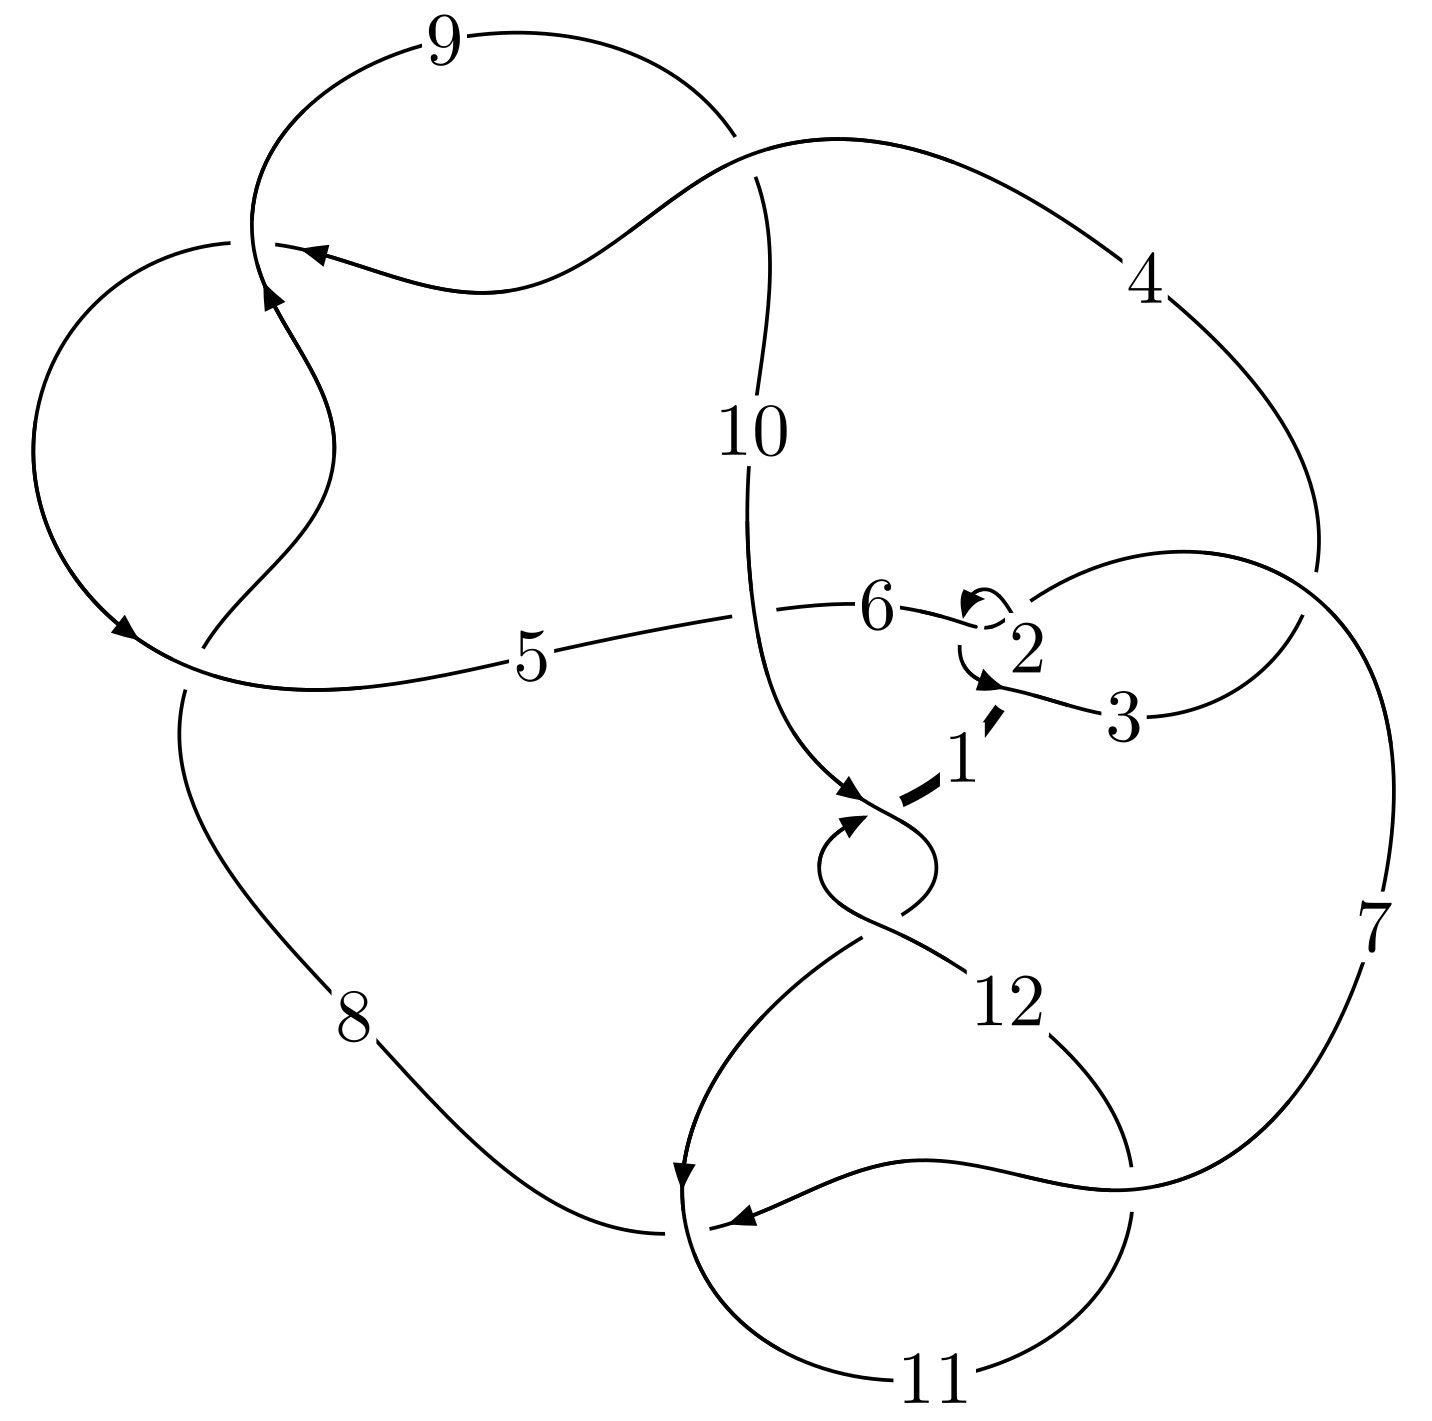
\includegraphics[width=112pt]{../../../GIT/diagram.site/Diagrams/png/2386_12n_0297.png}\\
\ \ \ A knot diagram\footnotemark}&
\allowdisplaybreaks
\textbf{Linearized knot diagam} \\
\cline{2-2}
 &
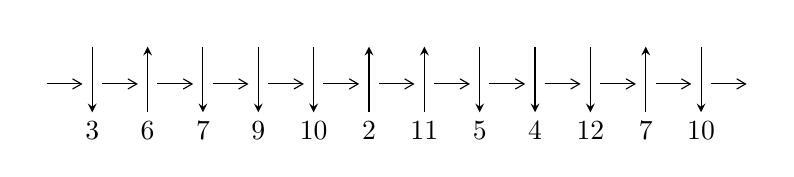
\begin{tikzpicture}[x=20pt, y=17pt]
	% nodes
	\node (C0) at (0, 0) {};
	\node (C1) at (1, 0) {};
	\node (C1U) at (1, +1) {};
	\node (C1D) at (1, -1) {3};

	\node (C2) at (2, 0) {};
	\node (C2U) at (2, +1) {};
	\node (C2D) at (2, -1) {6};

	\node (C3) at (3, 0) {};
	\node (C3U) at (3, +1) {};
	\node (C3D) at (3, -1) {7};

	\node (C4) at (4, 0) {};
	\node (C4U) at (4, +1) {};
	\node (C4D) at (4, -1) {9};

	\node (C5) at (5, 0) {};
	\node (C5U) at (5, +1) {};
	\node (C5D) at (5, -1) {10};

	\node (C6) at (6, 0) {};
	\node (C6U) at (6, +1) {};
	\node (C6D) at (6, -1) {2};

	\node (C7) at (7, 0) {};
	\node (C7U) at (7, +1) {};
	\node (C7D) at (7, -1) {11};

	\node (C8) at (8, 0) {};
	\node (C8U) at (8, +1) {};
	\node (C8D) at (8, -1) {5};

	\node (C9) at (9, 0) {};
	\node (C9U) at (9, +1) {};
	\node (C9D) at (9, -1) {4};

	\node (C10) at (10, 0) {};
	\node (C10U) at (10, +1) {};
	\node (C10D) at (10, -1) {12};

	\node (C11) at (11, 0) {};
	\node (C11U) at (11, +1) {};
	\node (C11D) at (11, -1) {7};

	\node (C12) at (12, 0) {};
	\node (C12U) at (12, +1) {};
	\node (C12D) at (12, -1) {10};
	\node (C13) at (13, 0) {};

	% arrows
	\draw[->,>={angle 60}]
	(C0) edge (C1) (C1) edge (C2) (C2) edge (C3) (C3) edge (C4) (C4) edge (C5) (C5) edge (C6) (C6) edge (C7) (C7) edge (C8) (C8) edge (C9) (C9) edge (C10) (C10) edge (C11) (C11) edge (C12) (C12) edge (C13) ;	\draw[->,>=stealth]
	(C1U) edge (C1D) (C2D) edge (C2U) (C3U) edge (C3D) (C4U) edge (C4D) (C5U) edge (C5D) (C6D) edge (C6U) (C7D) edge (C7U) (C8U) edge (C8D) (C9U) edge (C9D) (C10U) edge (C10D) (C11D) edge (C11U) (C12U) edge (C12D) ;
	\end{tikzpicture} \\
\hhline{~~} \\& 
\textbf{Solving Sequence} \\ \cline{2-2} 
 &
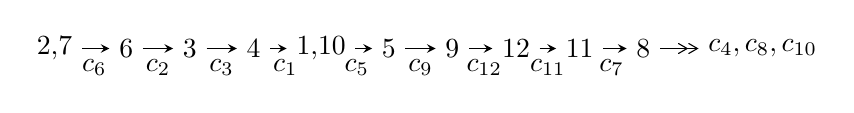
\begin{tikzpicture}[x=23pt, y=7pt]
	% node
	\node (A0) at (-1/8, 0) {2,7};
	\node (A1) at (1, 0) {6};
	\node (A2) at (2, 0) {3};
	\node (A3) at (3, 0) {4};
	\node (A4) at (65/16, 0) {1,10};
	\node (A5) at (41/8, 0) {5};
	\node (A6) at (49/8, 0) {9};
	\node (A7) at (57/8, 0) {12};
	\node (A8) at (65/8, 0) {11};
	\node (A9) at (73/8, 0) {8};
	\node (C1) at (1/2, -1) {$c_{6}$};
	\node (C2) at (3/2, -1) {$c_{2}$};
	\node (C3) at (5/2, -1) {$c_{3}$};
	\node (C4) at (7/2, -1) {$c_{1}$};
	\node (C5) at (37/8, -1) {$c_{5}$};
	\node (C6) at (45/8, -1) {$c_{9}$};
	\node (C7) at (53/8, -1) {$c_{12}$};
	\node (C8) at (61/8, -1) {$c_{11}$};
	\node (C9) at (69/8, -1) {$c_{7}$};
	\node (A10) at (11, 0) {$c_{4},c_{8},c_{10}$};

	% edge
	\draw[->,>=stealth]	
	(A0) edge (A1) (A1) edge (A2) (A2) edge (A3) (A3) edge (A4) (A4) edge (A5) (A5) edge (A6) (A6) edge (A7) (A7) edge (A8) (A8) edge (A9) ;
	\draw[->>,>={angle 60}]	
	(A9) edge (A10);
\end{tikzpicture} \\ 

\end{tabular} \\

\footnotetext{
The image of knot diagram is generated by the software ``\textbf{Draw programme}" developed by Andrew Bartholomew(\url{http://www.layer8.co.uk/maths/draw/index.htm\#Running-draw}), where we modified some parts for our purpose(\url{https://github.com/CATsTAILs/LinksPainter}).
}\phantom \\ \newline 
\centering \textbf{Ideals for irreducible components\footnotemark of $X_{\text{par}}$} 
 
\begin{align*}
I^u_{1}&=\langle 
- u^3+b- u,\;u^{13}- u^{12}+5 u^{11}-4 u^{10}+10 u^9-7 u^8+7 u^7-4 u^6-4 u^5+2 u^4-5 u^3+3 u^2+2 a+u+1,\\
\phantom{I^u_{1}}&\phantom{= \langle  }u^{17}- u^{16}+\cdots- u+1\rangle \\
I^u_{2}&=\langle 
-6.01027\times10^{15} u^{41}+4.38628\times10^{15} u^{40}+\cdots+4.85875\times10^{15} b-1.83034\times10^{16},\\
\phantom{I^u_{2}}&\phantom{= \langle  }2907486392199263 u^{41}-6406067892977536 u^{40}+\cdots+2242499937318462 a+3116730258713323,\\
\phantom{I^u_{2}}&\phantom{= \langle  }u^{42}-2 u^{41}+\cdots-13 u+3\rangle \\
I^u_{3}&=\langle 
b+u+1,\;a^2-2 a-2 u-1,\;u^2+u+1\rangle \\
I^u_{4}&=\langle 
b+u-1,\;a+1,\;u^2- u+1\rangle \\
I^u_{5}&=\langle 
b- u,\;a^2+2 a u+2 a- u-2,\;u^2+u+1\rangle \\
I^u_{6}&=\langle 
b- u,\;a+u-1,\;u^2- u+1\rangle \\
\\
\end{align*}
\raggedright * 6 irreducible components of $\dim_{\mathbb{C}}=0$, with total 71 representations.\\
\footnotetext{All coefficients of polynomials are rational numbers. But the coefficients are sometimes approximated in decimal forms when there is not enough margin.}
\newpage
\renewcommand{\arraystretch}{1}
\centering \section*{I. $I^u_{1}= \langle - u^3+b- u,\;u^{13}- u^{12}+\cdots+2 a+1,\;u^{17}- u^{16}+\cdots- u+1 \rangle$}
\flushleft \textbf{(i) Arc colorings}\\
\begin{tabular}{m{7pt} m{180pt} m{7pt} m{180pt} }
\flushright $a_{2}=$&$\begin{pmatrix}0\\u\end{pmatrix}$ \\
\flushright $a_{7}=$&$\begin{pmatrix}1\\0\end{pmatrix}$ \\
\flushright $a_{6}=$&$\begin{pmatrix}1\\u^2\end{pmatrix}$ \\
\flushright $a_{3}=$&$\begin{pmatrix}u\\u^3+u\end{pmatrix}$ \\
\flushright $a_{4}=$&$\begin{pmatrix}- u^3\\u^3+u\end{pmatrix}$ \\
\flushright $a_{1}=$&$\begin{pmatrix}u^3\\u^5+u^3+u\end{pmatrix}$ \\
\flushright $a_{10}=$&$\begin{pmatrix}-\frac{1}{2} u^{13}+\frac{1}{2} u^{12}+\cdots-\frac{1}{2} u-\frac{1}{2}\\u^3+u\end{pmatrix}$ \\
\flushright $a_{5}=$&$\begin{pmatrix}u^{16}- u^{15}+\cdots- u+\frac{3}{2}\\\frac{1}{2} u^{14}-\frac{1}{2} u^{13}+\cdots-\frac{1}{2} u^2+\frac{1}{2} u\end{pmatrix}$ \\
\flushright $a_{9}=$&$\begin{pmatrix}\frac{1}{2} u^{15}-\frac{1}{2} u^{14}+\cdots-\frac{1}{2} u-\frac{1}{2}\\-\frac{1}{2} u^{15}+\frac{1}{2} u^{14}+\cdots+\frac{3}{2} u-\frac{1}{2}\end{pmatrix}$ \\
\flushright $a_{12}=$&$\begin{pmatrix}\frac{1}{2} u^{15}-\frac{1}{2} u^{14}+\cdots+\frac{3}{2} u^3+\frac{1}{2} u^2\\u\end{pmatrix}$ \\
\flushright $a_{11}=$&$\begin{pmatrix}\frac{1}{2} u^{15}-\frac{1}{2} u^{14}+\cdots+\frac{1}{2} u^2- u\\u\end{pmatrix}$ \\
\flushright $a_{8}=$&$\begin{pmatrix}-\frac{1}{2} u^{16}+\frac{1}{2} u^{15}+\cdots+u^2+1\\- u^2\end{pmatrix}$\\&\end{tabular}
\flushleft \textbf{(ii) Obstruction class $= -1$}\\~\\
\flushleft \textbf{(iii) Cusp Shapes $= -5 u^{16}+2 u^{15}-24 u^{14}+5 u^{13}-50 u^{12}+5 u^{11}-42 u^{10}-3 u^9+8 u^8+33 u^6+4 u^5+8 u^4-4 u^3-11 u^2-8 u-6$}\\~\\
\newpage\renewcommand{\arraystretch}{1}
\flushleft \textbf{(iv) u-Polynomials at the component}\newline \\
\begin{tabular}{m{50pt}|m{274pt}}
Crossings & \hspace{64pt}u-Polynomials at each crossing \\
\hline $$\begin{aligned}c_{1},c_{10},c_{12}\end{aligned}$$&$\begin{aligned}
&u^{17}+11 u^{16}+\cdots-7 u-1
\end{aligned}$\\
\hline $$\begin{aligned}c_{2},c_{6},c_{7}\\c_{11}\end{aligned}$$&$\begin{aligned}
&u^{17}- u^{16}+\cdots- u+1
\end{aligned}$\\
\hline $$\begin{aligned}c_{3}\end{aligned}$$&$\begin{aligned}
&u^{17}+u^{16}+\cdots+u+1
\end{aligned}$\\
\hline $$\begin{aligned}c_{4},c_{8},c_{9}\end{aligned}$$&$\begin{aligned}
&u^{17}+5 u^{16}+\cdots+24 u+4
\end{aligned}$\\
\hline $$\begin{aligned}c_{5}\end{aligned}$$&$\begin{aligned}
&u^{17}-5 u^{16}+\cdots+32 u+356
\end{aligned}$\\
\hline
\end{tabular}\\~\\
\newpage\renewcommand{\arraystretch}{1}
\flushleft \textbf{(v) Riley Polynomials at the component}\newline \\
\begin{tabular}{m{50pt}|m{274pt}}
Crossings & \hspace{64pt}Riley Polynomials at each crossing \\
\hline $$\begin{aligned}c_{1},c_{10},c_{12}\end{aligned}$$&$\begin{aligned}
&y^{17}-5 y^{16}+\cdots+y-1
\end{aligned}$\\
\hline $$\begin{aligned}c_{2},c_{6},c_{7}\\c_{11}\end{aligned}$$&$\begin{aligned}
&y^{17}+11 y^{16}+\cdots-7 y-1
\end{aligned}$\\
\hline $$\begin{aligned}c_{3}\end{aligned}$$&$\begin{aligned}
&y^{17}-21 y^{16}+\cdots-7 y-1
\end{aligned}$\\
\hline $$\begin{aligned}c_{4},c_{8},c_{9}\end{aligned}$$&$\begin{aligned}
&y^{17}+15 y^{16}+\cdots-32 y-16
\end{aligned}$\\
\hline $$\begin{aligned}c_{5}\end{aligned}$$&$\begin{aligned}
&y^{17}-5 y^{16}+\cdots-685344 y-126736
\end{aligned}$\\
\hline
\end{tabular}\\~\\
\newpage\flushleft \textbf{(vi) Complex Volumes and Cusp Shapes}
$$\begin{array}{c|c|c}  
\text{Solutions to }I^u_{1}& \I (\text{vol} + \sqrt{-1}CS) & \text{Cusp shape}\\
 \hline 
\begin{aligned}
u &= -0.322943 + 1.038240 I \\
a &= -1.76695 - 1.17117 I \\
b &= \phantom{-}0.687713 + 0.243922 I\end{aligned}
 & \phantom{-}2.86633 - 4.06837 I & -7.21746 + 4.92513 I \\ \hline\begin{aligned}
u &= -0.322943 - 1.038240 I \\
a &= -1.76695 + 1.17117 I \\
b &= \phantom{-}0.687713 - 0.243922 I\end{aligned}
 & \phantom{-}2.86633 + 4.06837 I & -7.21746 - 4.92513 I \\ \hline\begin{aligned}
u &= \phantom{-}0.846972 + 0.190636 I \\
a &= \phantom{-}0.057316 + 0.298967 I \\
b &= \phantom{-}1.36222 + 0.59397 I\end{aligned}
 & \phantom{-}1.50690 - 4.21109 I & \phantom{-}0.87343 + 2.53739 I \\ \hline\begin{aligned}
u &= \phantom{-}0.846972 - 0.190636 I \\
a &= \phantom{-}0.057316 - 0.298967 I \\
b &= \phantom{-}1.36222 - 0.59397 I\end{aligned}
 & \phantom{-}1.50690 + 4.21109 I & \phantom{-}0.87343 - 2.53739 I \\ \hline\begin{aligned}
u &= \phantom{-}0.110349 + 1.142920 I \\
a &= \phantom{-}0.440223 - 0.492438 I \\
b &= -0.320742 - 0.308287 I\end{aligned}
 & -4.58609 + 2.21395 I & -10.42618 - 3.79439 I \\ \hline\begin{aligned}
u &= \phantom{-}0.110349 - 1.142920 I \\
a &= \phantom{-}0.440223 + 0.492438 I \\
b &= -0.320742 + 0.308287 I\end{aligned}
 & -4.58609 - 2.21395 I & -10.42618 + 3.79439 I \\ \hline\begin{aligned}
u &= -0.817813\phantom{ +0.000000I} \\
a &= -0.0448823\phantom{ +0.000000I} \\
b &= -1.36478\phantom{ +0.000000I}\end{aligned}
 & -2.55092\phantom{ +0.000000I} & -3.29090\phantom{ +0.000000I} \\ \hline\begin{aligned}
u &= -0.430215 + 0.605602 I \\
a &= \phantom{-}1.58821 - 0.32847 I \\
b &= -0.036492 + 0.719758 I\end{aligned}
 & \phantom{-}5.54966 - 2.41434 I & \phantom{-}1.92444 + 1.74579 I \\ \hline\begin{aligned}
u &= -0.430215 - 0.605602 I \\
a &= \phantom{-}1.58821 + 0.32847 I \\
b &= -0.036492 - 0.719758 I\end{aligned}
 & \phantom{-}5.54966 + 2.41434 I & \phantom{-}1.92444 - 1.74579 I \\ \hline\begin{aligned}
u &= \phantom{-}0.432341 + 1.261340 I \\
a &= \phantom{-}1.58526 + 0.60200 I \\
b &= -1.55038 - 0.03811 I\end{aligned}
 & -6.94626 + 4.33928 I & -7.37666 - 2.73345 I\\
 \hline 
 \end{array}$$\newpage$$\begin{array}{c|c|c}  
\text{Solutions to }I^u_{1}& \I (\text{vol} + \sqrt{-1}CS) & \text{Cusp shape}\\
 \hline 
\begin{aligned}
u &= \phantom{-}0.432341 - 1.261340 I \\
a &= \phantom{-}1.58526 - 0.60200 I \\
b &= -1.55038 + 0.03811 I\end{aligned}
 & -6.94626 - 4.33928 I & -7.37666 + 2.73345 I \\ \hline\begin{aligned}
u &= \phantom{-}0.581005 + 1.217160 I \\
a &= \phantom{-}1.92685 + 1.19674 I \\
b &= -1.80511 + 0.64658 I\end{aligned}
 & -4.4941 + 14.7863 I & -4.66375 - 8.62681 I \\ \hline\begin{aligned}
u &= \phantom{-}0.581005 - 1.217160 I \\
a &= \phantom{-}1.92685 - 1.19674 I \\
b &= -1.80511 - 0.64658 I\end{aligned}
 & -4.4941 - 14.7863 I & -4.66375 + 8.62681 I \\ \hline\begin{aligned}
u &= -0.523425 + 1.252060 I \\
a &= -1.77570 + 0.95237 I \\
b &= \phantom{-}1.79480 + 0.31837 I\end{aligned}
 & -9.65986 - 9.78843 I & -8.66609 + 6.57063 I \\ \hline\begin{aligned}
u &= -0.523425 - 1.252060 I \\
a &= -1.77570 - 0.95237 I \\
b &= \phantom{-}1.79480 - 0.31837 I\end{aligned}
 & -9.65986 + 9.78843 I & -8.66609 - 6.57063 I \\ \hline\begin{aligned}
u &= \phantom{-}0.214821 + 0.520126 I \\
a &= -0.532769 - 0.701691 I \\
b &= \phantom{-}0.050387 + 0.451424 I\end{aligned}
 & -0.232914 + 1.043600 I & -3.80228 - 6.41835 I \\ \hline\begin{aligned}
u &= \phantom{-}0.214821 - 0.520126 I \\
a &= -0.532769 + 0.701691 I \\
b &= \phantom{-}0.050387 - 0.451424 I\end{aligned}
 & -0.232914 - 1.043600 I & -3.80228 + 6.41835 I\\
 \hline 
 \end{array}$$\newpage\newpage\renewcommand{\arraystretch}{1}
\centering \section*{II. $I^u_{2}= \langle -6.01\times10^{15} u^{41}+4.39\times10^{15} u^{40}+\cdots+4.86\times10^{15} b-1.83\times10^{16},\;2.91\times10^{15} u^{41}-6.41\times10^{15} u^{40}+\cdots+2.24\times10^{15} a+3.12\times10^{15},\;u^{42}-2 u^{41}+\cdots-13 u+3 \rangle$}
\flushleft \textbf{(i) Arc colorings}\\
\begin{tabular}{m{7pt} m{180pt} m{7pt} m{180pt} }
\flushright $a_{2}=$&$\begin{pmatrix}0\\u\end{pmatrix}$ \\
\flushright $a_{7}=$&$\begin{pmatrix}1\\0\end{pmatrix}$ \\
\flushright $a_{6}=$&$\begin{pmatrix}1\\u^2\end{pmatrix}$ \\
\flushright $a_{3}=$&$\begin{pmatrix}u\\u^3+u\end{pmatrix}$ \\
\flushright $a_{4}=$&$\begin{pmatrix}- u^3\\u^3+u\end{pmatrix}$ \\
\flushright $a_{1}=$&$\begin{pmatrix}u^3\\u^5+u^3+u\end{pmatrix}$ \\
\flushright $a_{10}=$&$\begin{pmatrix}-1.29654 u^{41}+2.85666 u^{40}+\cdots-2.89896 u-1.38985\\1.23700 u^{41}-0.902758 u^{40}+\cdots-18.1061 u+3.76710\end{pmatrix}$ \\
\flushright $a_{5}=$&$\begin{pmatrix}-1.28722 u^{41}+4.62863 u^{40}+\cdots-72.8325 u+16.6384\\0.929780 u^{41}-2.10128 u^{40}+\cdots+4.35029 u+1.40533\end{pmatrix}$ \\
\flushright $a_{9}=$&$\begin{pmatrix}-0.801807 u^{41}+1.81747 u^{40}+\cdots+6.37909 u-3.86212\\0.263884 u^{41}+0.269109 u^{40}+\cdots-18.9125 u+3.93233\end{pmatrix}$ \\
\flushright $a_{12}=$&$\begin{pmatrix}-0.615799 u^{41}+0.348663 u^{40}+\cdots+35.1901 u-10.2810\\-0.211969 u^{41}+1.35987 u^{40}+\cdots-12.2107 u+0.682808\end{pmatrix}$ \\
\flushright $a_{11}=$&$\begin{pmatrix}-0.403831 u^{41}-1.01121 u^{40}+\cdots+47.4008 u-10.9638\\-0.211969 u^{41}+1.35987 u^{40}+\cdots-12.2107 u+0.682808\end{pmatrix}$ \\
\flushright $a_{8}=$&$\begin{pmatrix}-3.43389 u^{41}+6.89021 u^{40}+\cdots-2.02041 u-3.37620\\1.03167 u^{41}-1.32061 u^{40}+\cdots-1.13275 u+0.551934\end{pmatrix}$\\&\end{tabular}
\flushleft \textbf{(ii) Obstruction class $= -1$}\\~\\
\flushleft \textbf{(iii) Cusp Shapes $= \frac{14132658601726202}{4858749864190001} u^{41}-\frac{2000261855343520}{373749989553077} u^{40}+\cdots+\frac{110747832601789324}{4858749864190001} u-\frac{19778111821628499}{4858749864190001}$}\\~\\
\newpage\renewcommand{\arraystretch}{1}
\flushleft \textbf{(iv) u-Polynomials at the component}\newline \\
\begin{tabular}{m{50pt}|m{274pt}}
Crossings & \hspace{64pt}u-Polynomials at each crossing \\
\hline $$\begin{aligned}c_{1},c_{10},c_{12}\end{aligned}$$&$\begin{aligned}
&u^{42}+22 u^{41}+\cdots+59 u+9
\end{aligned}$\\
\hline $$\begin{aligned}c_{2},c_{6},c_{7}\\c_{11}\end{aligned}$$&$\begin{aligned}
&u^{42}-2 u^{41}+\cdots-13 u+3
\end{aligned}$\\
\hline $$\begin{aligned}c_{3}\end{aligned}$$&$\begin{aligned}
&u^{42}+2 u^{41}+\cdots-1001 u+375
\end{aligned}$\\
\hline $$\begin{aligned}c_{4},c_{8},c_{9}\end{aligned}$$&$\begin{aligned}
&(u^{21}-2 u^{20}+\cdots-4 u+2)^{2}
\end{aligned}$\\
\hline $$\begin{aligned}c_{5}\end{aligned}$$&$\begin{aligned}
&(u^{21}+2 u^{20}+\cdots-4 u+2)^{2}
\end{aligned}$\\
\hline
\end{tabular}\\~\\
\newpage\renewcommand{\arraystretch}{1}
\flushleft \textbf{(v) Riley Polynomials at the component}\newline \\
\begin{tabular}{m{50pt}|m{274pt}}
Crossings & \hspace{64pt}Riley Polynomials at each crossing \\
\hline $$\begin{aligned}c_{1},c_{10},c_{12}\end{aligned}$$&$\begin{aligned}
&y^{42}-2 y^{41}+\cdots-2329 y+81
\end{aligned}$\\
\hline $$\begin{aligned}c_{2},c_{6},c_{7}\\c_{11}\end{aligned}$$&$\begin{aligned}
&y^{42}+22 y^{41}+\cdots+59 y+9
\end{aligned}$\\
\hline $$\begin{aligned}c_{3}\end{aligned}$$&$\begin{aligned}
&y^{42}-26 y^{41}+\cdots+2152499 y+140625
\end{aligned}$\\
\hline $$\begin{aligned}c_{4},c_{8},c_{9}\end{aligned}$$&$\begin{aligned}
&(y^{21}+18 y^{20}+\cdots+16 y-4)^{2}
\end{aligned}$\\
\hline $$\begin{aligned}c_{5}\end{aligned}$$&$\begin{aligned}
&(y^{21}-22 y^{20}+\cdots+40 y-4)^{2}
\end{aligned}$\\
\hline
\end{tabular}\\~\\
\newpage\flushleft \textbf{(vi) Complex Volumes and Cusp Shapes}
$$\begin{array}{c|c|c}  
\text{Solutions to }I^u_{2}& \I (\text{vol} + \sqrt{-1}CS) & \text{Cusp shape}\\
 \hline 
\begin{aligned}
u &= -0.648340 + 0.786994 I \\
a &= \phantom{-}0.520796 + 0.410581 I \\
b &= \phantom{-}0.600235 + 0.207579 I\end{aligned}
 & \phantom{-}4.76959 - 2.48515 I & \phantom{-}1.90098 + 3.54281 I \\ \hline\begin{aligned}
u &= -0.648340 - 0.786994 I \\
a &= \phantom{-}0.520796 - 0.410581 I \\
b &= \phantom{-}0.600235 - 0.207579 I\end{aligned}
 & \phantom{-}4.76959 + 2.48515 I & \phantom{-}1.90098 - 3.54281 I \\ \hline\begin{aligned}
u &= -0.281169 + 0.918116 I \\
a &= \phantom{-}1.66079 + 0.03172 I \\
b &= -0.705944 - 1.191570 I\end{aligned}
 & -0.82885 - 3.61332 I & -9.58837 + 1.89402 I \\ \hline\begin{aligned}
u &= -0.281169 - 0.918116 I \\
a &= \phantom{-}1.66079 - 0.03172 I \\
b &= -0.705944 + 1.191570 I\end{aligned}
 & -0.82885 + 3.61332 I & -9.58837 - 1.89402 I \\ \hline\begin{aligned}
u &= \phantom{-}0.919345 + 0.237233 I \\
a &= \phantom{-}0.139375 - 0.118273 I \\
b &= -1.65616 - 0.52114 I\end{aligned}
 & -1.52142 - 9.31938 I & -2.21398 + 5.58015 I \\ \hline\begin{aligned}
u &= \phantom{-}0.919345 - 0.237233 I \\
a &= \phantom{-}0.139375 + 0.118273 I \\
b &= -1.65616 + 0.52114 I\end{aligned}
 & -1.52142 + 9.31938 I & -2.21398 - 5.58015 I \\ \hline\begin{aligned}
u &= -0.918649 + 0.104898 I \\
a &= -0.159545 + 0.217864 I \\
b &= \phantom{-}1.52694 - 0.17361 I\end{aligned}
 & -6.16843 + 4.59035 I & -6.34834 - 3.42334 I \\ \hline\begin{aligned}
u &= -0.918649 - 0.104898 I \\
a &= -0.159545 - 0.217864 I \\
b &= \phantom{-}1.52694 + 0.17361 I\end{aligned}
 & -6.16843 - 4.59035 I & -6.34834 + 3.42334 I \\ \hline\begin{aligned}
u &= -0.746719 + 0.798648 I \\
a &= \phantom{-}0.124923 - 0.315475 I \\
b &= -1.083540 - 0.394401 I\end{aligned}
 & \phantom{-}2.13930 - 6.31791 I & -2.69400 + 7.27088 I \\ \hline\begin{aligned}
u &= -0.746719 - 0.798648 I \\
a &= \phantom{-}0.124923 + 0.315475 I \\
b &= -1.083540 + 0.394401 I\end{aligned}
 & \phantom{-}2.13930 + 6.31791 I & -2.69400 - 7.27088 I\\
 \hline 
 \end{array}$$\newpage$$\begin{array}{c|c|c}  
\text{Solutions to }I^u_{2}& \I (\text{vol} + \sqrt{-1}CS) & \text{Cusp shape}\\
 \hline 
\begin{aligned}
u &= \phantom{-}0.896010 + 0.063848 I \\
a &= \phantom{-}0.148702 - 0.571049 I \\
b &= -1.197580 - 0.165877 I\end{aligned}
 & -2.87260 - 0.28571 I & -3.90381 + 0.09482 I \\ \hline\begin{aligned}
u &= \phantom{-}0.896010 - 0.063848 I \\
a &= \phantom{-}0.148702 + 0.571049 I \\
b &= -1.197580 + 0.165877 I\end{aligned}
 & -2.87260 + 0.28571 I & -3.90381 - 0.09482 I \\ \hline\begin{aligned}
u &= \phantom{-}0.616574 + 0.917444 I \\
a &= -0.466225 + 0.312796 I \\
b &= \phantom{-}0.407626 - 0.361948 I\end{aligned}
 & -0.82885 + 3.61332 I & -9.58837 - 1.89402 I \\ \hline\begin{aligned}
u &= \phantom{-}0.616574 - 0.917444 I \\
a &= -0.466225 - 0.312796 I \\
b &= \phantom{-}0.407626 + 0.361948 I\end{aligned}
 & -0.82885 - 3.61332 I & -9.58837 + 1.89402 I \\ \hline\begin{aligned}
u &= -0.707790 + 0.857193 I \\
a &= -0.264002 - 1.060620 I \\
b &= -0.934767 + 0.363773 I\end{aligned}
 & \phantom{-}1.95965 + 0.82852 I & -3.22814 - 1.28551 I \\ \hline\begin{aligned}
u &= -0.707790 - 0.857193 I \\
a &= -0.264002 + 1.060620 I \\
b &= -0.934767 - 0.363773 I\end{aligned}
 & \phantom{-}1.95965 - 0.82852 I & -3.22814 + 1.28551 I \\ \hline\begin{aligned}
u &= -0.553188 + 0.964414 I \\
a &= \phantom{-}1.11387 + 1.08458 I \\
b &= \phantom{-}0.028624 - 0.375859 I\end{aligned}
 & \phantom{-}4.51229 - 1.78805 I & -2.74245 + 3.28020 I \\ \hline\begin{aligned}
u &= -0.553188 - 0.964414 I \\
a &= \phantom{-}1.11387 - 1.08458 I \\
b &= \phantom{-}0.028624 + 0.375859 I\end{aligned}
 & \phantom{-}4.51229 + 1.78805 I & -2.74245 - 3.28020 I \\ \hline\begin{aligned}
u &= \phantom{-}0.405897 + 1.075130 I \\
a &= \phantom{-}0.742962 - 1.081300 I \\
b &= \phantom{-}0.49784 + 1.51562 I\end{aligned}
 & \phantom{-}1.95965 + 0.82852 I & -3.22814 - 1.28551 I \\ \hline\begin{aligned}
u &= \phantom{-}0.405897 - 1.075130 I \\
a &= \phantom{-}0.742962 + 1.081300 I \\
b &= \phantom{-}0.49784 - 1.51562 I\end{aligned}
 & \phantom{-}1.95965 - 0.82852 I & -3.22814 + 1.28551 I\\
 \hline 
 \end{array}$$\newpage$$\begin{array}{c|c|c}  
\text{Solutions to }I^u_{2}& \I (\text{vol} + \sqrt{-1}CS) & \text{Cusp shape}\\
 \hline 
\begin{aligned}
u &= \phantom{-}0.515102 + 0.670364 I \\
a &= -0.086404 - 0.577180 I \\
b &= \phantom{-}0.058588 + 0.436947 I\end{aligned}
 & -0.099396 + 1.054050 I & -5.09416 - 5.72302 I \\ \hline\begin{aligned}
u &= \phantom{-}0.515102 - 0.670364 I \\
a &= -0.086404 + 0.577180 I \\
b &= \phantom{-}0.058588 - 0.436947 I\end{aligned}
 & -0.099396 - 1.054050 I & -5.09416 + 5.72302 I \\ \hline\begin{aligned}
u &= \phantom{-}0.438792 + 1.104820 I \\
a &= -1.41623 + 0.50848 I \\
b &= \phantom{-}0.26578 - 1.62519 I\end{aligned}
 & \phantom{-}2.13930 + 6.31791 I & -2.69400 - 7.27088 I \\ \hline\begin{aligned}
u &= \phantom{-}0.438792 - 1.104820 I \\
a &= -1.41623 - 0.50848 I \\
b &= \phantom{-}0.26578 + 1.62519 I\end{aligned}
 & \phantom{-}2.13930 - 6.31791 I & -2.69400 + 7.27088 I \\ \hline\begin{aligned}
u &= \phantom{-}0.352371 + 1.227840 I \\
a &= -1.56964 - 0.94140 I \\
b &= \phantom{-}1.60440 + 0.21737 I\end{aligned}
 & -2.87260 - 0.28571 I & -4.00000 + 0. I\phantom{ +0.000000I} \\ \hline\begin{aligned}
u &= \phantom{-}0.352371 - 1.227840 I \\
a &= -1.56964 + 0.94140 I \\
b &= \phantom{-}1.60440 - 0.21737 I\end{aligned}
 & -2.87260 + 0.28571 I & -4.00000 + 0. I\phantom{ +0.000000I} \\ \hline\begin{aligned}
u &= -0.184003 + 0.671383 I \\
a &= -1.095080 - 0.579917 I \\
b &= -0.042669 + 0.902715 I\end{aligned}
 & -0.099396 + 1.054050 I & -5.09416 - 5.72302 I \\ \hline\begin{aligned}
u &= -0.184003 - 0.671383 I \\
a &= -1.095080 + 0.579917 I \\
b &= -0.042669 - 0.902715 I\end{aligned}
 & -0.099396 - 1.054050 I & -5.09416 + 5.72302 I \\ \hline\begin{aligned}
u &= -0.463537 + 1.225960 I \\
a &= \phantom{-}1.72317 - 0.93419 I \\
b &= -1.66359 - 0.36932 I\end{aligned}
 & -6.16843 - 4.59035 I & \phantom{-0.000000 } 0 \\ \hline\begin{aligned}
u &= -0.463537 - 1.225960 I \\
a &= \phantom{-}1.72317 + 0.93419 I \\
b &= -1.66359 + 0.36932 I\end{aligned}
 & -6.16843 + 4.59035 I & \phantom{-0.000000 } 0\\
 \hline 
 \end{array}$$\newpage$$\begin{array}{c|c|c}  
\text{Solutions to }I^u_{2}& \I (\text{vol} + \sqrt{-1}CS) & \text{Cusp shape}\\
 \hline 
\begin{aligned}
u &= -0.073463 + 0.681917 I \\
a &= -2.84879 - 0.54672 I \\
b &= \phantom{-}0.821077 - 0.952800 I\end{aligned}
 & \phantom{-}4.51229 + 1.78805 I & -2.74245 - 3.28020 I \\ \hline\begin{aligned}
u &= -0.073463 - 0.681917 I \\
a &= -2.84879 + 0.54672 I \\
b &= \phantom{-}0.821077 + 0.952800 I\end{aligned}
 & \phantom{-}4.51229 - 1.78805 I & -2.74245 + 3.28020 I \\ \hline\begin{aligned}
u &= \phantom{-}0.542292 + 1.203890 I \\
a &= -1.84110 - 0.94344 I \\
b &= \phantom{-}1.54115 - 0.82541 I\end{aligned}
 & -1.52142 + 9.31938 I & \phantom{-0.000000 } 0. - 5.58015 I \\ \hline\begin{aligned}
u &= \phantom{-}0.542292 - 1.203890 I \\
a &= -1.84110 + 0.94344 I \\
b &= \phantom{-}1.54115 + 0.82541 I\end{aligned}
 & -1.52142 - 9.31938 I & \phantom{-0.000000 -}0. + 5.58015 I \\ \hline\begin{aligned}
u &= \phantom{-}0.301624 + 1.287530 I \\
a &= \phantom{-}1.83725 + 0.98743 I \\
b &= -1.71923 - 0.20551 I\end{aligned}
 & -6.49606 - 5.29485 I & \phantom{-0.000000 } 0 \\ \hline\begin{aligned}
u &= \phantom{-}0.301624 - 1.287530 I \\
a &= \phantom{-}1.83725 - 0.98743 I \\
b &= -1.71923 + 0.20551 I\end{aligned}
 & -6.49606 + 5.29485 I & \phantom{-0.000000 } 0 \\ \hline\begin{aligned}
u &= \phantom{-}0.495316 + 1.253840 I \\
a &= \phantom{-}1.39824 + 0.99998 I \\
b &= -1.170980 + 0.495445 I\end{aligned}
 & -6.49606 + 5.29485 I & \phantom{-0.000000 } 0 \\ \hline\begin{aligned}
u &= \phantom{-}0.495316 - 1.253840 I \\
a &= \phantom{-}1.39824 - 0.99998 I \\
b &= -1.170980 - 0.495445 I\end{aligned}
 & -6.49606 - 5.29485 I & \phantom{-0.000000 } 0 \\ \hline\begin{aligned}
u &= -0.404607 + 1.286580 I \\
a &= -1.64330 + 1.00540 I \\
b &= \phantom{-}1.53839 + 0.21123 I\end{aligned}
 & -10.5274\phantom{ +0.000000I} & \phantom{-0.000000 } 0 \\ \hline\begin{aligned}
u &= -0.404607 - 1.286580 I \\
a &= -1.64330 - 1.00540 I \\
b &= \phantom{-}1.53839 - 0.21123 I\end{aligned}
 & -10.5274\phantom{ +0.000000I} & \phantom{-0.000000 } 0\\
 \hline 
 \end{array}$$\newpage$$\begin{array}{c|c|c}  
\text{Solutions to }I^u_{2}& \I (\text{vol} + \sqrt{-1}CS) & \text{Cusp shape}\\
 \hline 
\begin{aligned}
u &= \phantom{-}0.498140 + 0.119986 I \\
a &= \phantom{-}0.81356 + 1.59996 I \\
b &= \phantom{-}0.283799 + 1.291990 I\end{aligned}
 & \phantom{-}4.76959 - 2.48515 I & \phantom{-}1.90098 + 3.54281 I \\ \hline\begin{aligned}
u &= \phantom{-}0.498140 - 0.119986 I \\
a &= \phantom{-}0.81356 - 1.59996 I \\
b &= \phantom{-}0.283799 - 1.291990 I\end{aligned}
 & \phantom{-}4.76959 + 2.48515 I & \phantom{-}1.90098 - 3.54281 I\\
 \hline 
 \end{array}$$\newpage\newpage\renewcommand{\arraystretch}{1}
\centering \section*{III. $I^u_{3}= \langle b+u+1,\;a^2-2 a-2 u-1,\;u^2+u+1 \rangle$}
\flushleft \textbf{(i) Arc colorings}\\
\begin{tabular}{m{7pt} m{180pt} m{7pt} m{180pt} }
\flushright $a_{2}=$&$\begin{pmatrix}0\\u\end{pmatrix}$ \\
\flushright $a_{7}=$&$\begin{pmatrix}1\\0\end{pmatrix}$ \\
\flushright $a_{6}=$&$\begin{pmatrix}1\\- u-1\end{pmatrix}$ \\
\flushright $a_{3}=$&$\begin{pmatrix}u\\u+1\end{pmatrix}$ \\
\flushright $a_{4}=$&$\begin{pmatrix}-1\\u+1\end{pmatrix}$ \\
\flushright $a_{1}=$&$\begin{pmatrix}1\\0\end{pmatrix}$ \\
\flushright $a_{10}=$&$\begin{pmatrix}a\\- u-1\end{pmatrix}$ \\
\flushright $a_{5}=$&$\begin{pmatrix}- a u- a- u+2\\a u-2 u-1\end{pmatrix}$ \\
\flushright $a_{9}=$&$\begin{pmatrix}a u+2 a- u-1\\- a u-1\end{pmatrix}$ \\
\flushright $a_{12}=$&$\begin{pmatrix}a u+a+1\\- u\end{pmatrix}$ \\
\flushright $a_{11}=$&$\begin{pmatrix}a u+a+u+1\\- u\end{pmatrix}$ \\
\flushright $a_{8}=$&$\begin{pmatrix}- a\\u+1\end{pmatrix}$\\&\end{tabular}
\flushleft \textbf{(ii) Obstruction class $= 1$}\\~\\
\flushleft \textbf{(iii) Cusp Shapes $= 8 u+4$}\\~\\
\newpage\renewcommand{\arraystretch}{1}
\flushleft \textbf{(iv) u-Polynomials at the component}\newline \\
\begin{tabular}{m{50pt}|m{274pt}}
Crossings & \hspace{64pt}u-Polynomials at each crossing \\
\hline $$\begin{aligned}c_{1},c_{2},c_{7}\\c_{10}\end{aligned}$$&$\begin{aligned}
&(u^2- u+1)^2
\end{aligned}$\\
\hline $$\begin{aligned}c_{3},c_{6},c_{11}\\c_{12}\end{aligned}$$&$\begin{aligned}
&(u^2+u+1)^2
\end{aligned}$\\
\hline $$\begin{aligned}c_{4},c_{5},c_{8}\\c_{9}\end{aligned}$$&$\begin{aligned}
&(u^2+2)^2
\end{aligned}$\\
\hline
\end{tabular}\\~\\
\newpage\renewcommand{\arraystretch}{1}
\flushleft \textbf{(v) Riley Polynomials at the component}\newline \\
\begin{tabular}{m{50pt}|m{274pt}}
Crossings & \hspace{64pt}Riley Polynomials at each crossing \\
\hline $$\begin{aligned}c_{1},c_{2},c_{3}\\c_{6},c_{7},c_{10}\\c_{11},c_{12}\end{aligned}$$&$\begin{aligned}
&(y^2+y+1)^2
\end{aligned}$\\
\hline $$\begin{aligned}c_{4},c_{5},c_{8}\\c_{9}\end{aligned}$$&$\begin{aligned}
&(y+2)^4
\end{aligned}$\\
\hline
\end{tabular}\\~\\
\newpage\flushleft \textbf{(vi) Complex Volumes and Cusp Shapes}
$$\begin{array}{c|c|c}  
\text{Solutions to }I^u_{3}& \I (\text{vol} + \sqrt{-1}CS) & \text{Cusp shape}\\
 \hline 
\begin{aligned}
u &= -0.500000 + 0.866025 I \\
a &= -0.224745 - 0.707107 I \\
b &= -0.500000 - 0.866025 I\end{aligned}
 & \phantom{-}4.93480 - 4.05977 I & \phantom{-0.000000 -}0. + 6.92820 I \\ \hline\begin{aligned}
u &= -0.500000 + 0.866025 I \\
a &= \phantom{-}2.22474 + 0.70711 I \\
b &= -0.500000 - 0.866025 I\end{aligned}
 & \phantom{-}4.93480 - 4.05977 I & \phantom{-0.000000 -}0. + 6.92820 I \\ \hline\begin{aligned}
u &= -0.500000 - 0.866025 I \\
a &= -0.224745 + 0.707107 I \\
b &= -0.500000 + 0.866025 I\end{aligned}
 & \phantom{-}4.93480 + 4.05977 I & \phantom{-0.000000 } 0. - 6.92820 I \\ \hline\begin{aligned}
u &= -0.500000 - 0.866025 I \\
a &= \phantom{-}2.22474 - 0.70711 I \\
b &= -0.500000 + 0.866025 I\end{aligned}
 & \phantom{-}4.93480 + 4.05977 I & \phantom{-0.000000 } 0. - 6.92820 I\\
 \hline 
 \end{array}$$\newpage\newpage\renewcommand{\arraystretch}{1}
\centering \section*{IV. $I^u_{4}= \langle b+u-1,\;a+1,\;u^2- u+1 \rangle$}
\flushleft \textbf{(i) Arc colorings}\\
\begin{tabular}{m{7pt} m{180pt} m{7pt} m{180pt} }
\flushright $a_{2}=$&$\begin{pmatrix}0\\u\end{pmatrix}$ \\
\flushright $a_{7}=$&$\begin{pmatrix}1\\0\end{pmatrix}$ \\
\flushright $a_{6}=$&$\begin{pmatrix}1\\u-1\end{pmatrix}$ \\
\flushright $a_{3}=$&$\begin{pmatrix}u\\u-1\end{pmatrix}$ \\
\flushright $a_{4}=$&$\begin{pmatrix}1\\u-1\end{pmatrix}$ \\
\flushright $a_{1}=$&$\begin{pmatrix}-1\\0\end{pmatrix}$ \\
\flushright $a_{10}=$&$\begin{pmatrix}-1\\- u+1\end{pmatrix}$ \\
\flushright $a_{5}=$&$\begin{pmatrix}1\\u-1\end{pmatrix}$ \\
\flushright $a_{9}=$&$\begin{pmatrix}-1\\- u+1\end{pmatrix}$ \\
\flushright $a_{12}=$&$\begin{pmatrix}u-2\\- u\end{pmatrix}$ \\
\flushright $a_{11}=$&$\begin{pmatrix}2 u-2\\- u\end{pmatrix}$ \\
\flushright $a_{8}=$&$\begin{pmatrix}-1\\- u+1\end{pmatrix}$\\&\end{tabular}
\flushleft \textbf{(ii) Obstruction class $= 1$}\\~\\
\flushleft \textbf{(iii) Cusp Shapes $= -8 u+4$}\\~\\
\newpage\renewcommand{\arraystretch}{1}
\flushleft \textbf{(iv) u-Polynomials at the component}\newline \\
\begin{tabular}{m{50pt}|m{274pt}}
Crossings & \hspace{64pt}u-Polynomials at each crossing \\
\hline $$\begin{aligned}c_{1},c_{3},c_{6}\\c_{10},c_{11}\end{aligned}$$&$\begin{aligned}
&u^2- u+1
\end{aligned}$\\
\hline $$\begin{aligned}c_{2},c_{7},c_{12}\end{aligned}$$&$\begin{aligned}
&u^2+u+1
\end{aligned}$\\
\hline $$\begin{aligned}c_{4},c_{5},c_{8}\\c_{9}\end{aligned}$$&$\begin{aligned}
&u^2
\end{aligned}$\\
\hline
\end{tabular}\\~\\
\newpage\renewcommand{\arraystretch}{1}
\flushleft \textbf{(v) Riley Polynomials at the component}\newline \\
\begin{tabular}{m{50pt}|m{274pt}}
Crossings & \hspace{64pt}Riley Polynomials at each crossing \\
\hline $$\begin{aligned}c_{1},c_{2},c_{3}\\c_{6},c_{7},c_{10}\\c_{11},c_{12}\end{aligned}$$&$\begin{aligned}
&y^2+y+1
\end{aligned}$\\
\hline $$\begin{aligned}c_{4},c_{5},c_{8}\\c_{9}\end{aligned}$$&$\begin{aligned}
&y^2
\end{aligned}$\\
\hline
\end{tabular}\\~\\
\newpage\flushleft \textbf{(vi) Complex Volumes and Cusp Shapes}
$$\begin{array}{c|c|c}  
\text{Solutions to }I^u_{4}& \I (\text{vol} + \sqrt{-1}CS) & \text{Cusp shape}\\
 \hline 
\begin{aligned}
u &= \phantom{-}0.500000 + 0.866025 I \\
a &= -1.00000\phantom{ +0.000000I} \\
b &= \phantom{-}0.500000 - 0.866025 I\end{aligned}
 & \phantom{-0.000000 -}4.05977 I & \phantom{-0.000000 } 0. - 6.92820 I \\ \hline\begin{aligned}
u &= \phantom{-}0.500000 - 0.866025 I \\
a &= -1.00000\phantom{ +0.000000I} \\
b &= \phantom{-}0.500000 + 0.866025 I\end{aligned}
 & \phantom{-0.000000 } -4.05977 I & \phantom{-0.000000 -}0. + 6.92820 I\\
 \hline 
 \end{array}$$\newpage\newpage\renewcommand{\arraystretch}{1}
\centering \section*{V. $I^u_{5}= \langle b- u,\;a^2+2 a u+2 a- u-2,\;u^2+u+1 \rangle$}
\flushleft \textbf{(i) Arc colorings}\\
\begin{tabular}{m{7pt} m{180pt} m{7pt} m{180pt} }
\flushright $a_{2}=$&$\begin{pmatrix}0\\u\end{pmatrix}$ \\
\flushright $a_{7}=$&$\begin{pmatrix}1\\0\end{pmatrix}$ \\
\flushright $a_{6}=$&$\begin{pmatrix}1\\- u-1\end{pmatrix}$ \\
\flushright $a_{3}=$&$\begin{pmatrix}u\\u+1\end{pmatrix}$ \\
\flushright $a_{4}=$&$\begin{pmatrix}-1\\u+1\end{pmatrix}$ \\
\flushright $a_{1}=$&$\begin{pmatrix}1\\0\end{pmatrix}$ \\
\flushright $a_{10}=$&$\begin{pmatrix}a\\u\end{pmatrix}$ \\
\flushright $a_{5}=$&$\begin{pmatrix}a u-2 u\\a\end{pmatrix}$ \\
\flushright $a_{9}=$&$\begin{pmatrix}a u+2 a+u\\- a u+u+1\end{pmatrix}$ \\
\flushright $a_{12}=$&$\begin{pmatrix}- a u+1\\u+1\end{pmatrix}$ \\
\flushright $a_{11}=$&$\begin{pmatrix}- a u- u\\u+1\end{pmatrix}$ \\
\flushright $a_{8}=$&$\begin{pmatrix}- a\\- u\end{pmatrix}$\\&\end{tabular}
\flushleft \textbf{(ii) Obstruction class $= 1$}\\~\\
\flushleft \textbf{(iii) Cusp Shapes $= 0$}\\~\\
\newpage\renewcommand{\arraystretch}{1}
\flushleft \textbf{(iv) u-Polynomials at the component}\newline \\
\begin{tabular}{m{50pt}|m{274pt}}
Crossings & \hspace{64pt}u-Polynomials at each crossing \\
\hline $$\begin{aligned}c_{1},c_{2},c_{7}\\c_{10}\end{aligned}$$&$\begin{aligned}
&(u^2- u+1)^2
\end{aligned}$\\
\hline $$\begin{aligned}c_{3},c_{6},c_{11}\\c_{12}\end{aligned}$$&$\begin{aligned}
&(u^2+u+1)^2
\end{aligned}$\\
\hline $$\begin{aligned}c_{4},c_{5},c_{8}\\c_{9}\end{aligned}$$&$\begin{aligned}
&(u^2+2)^2
\end{aligned}$\\
\hline
\end{tabular}\\~\\
\newpage\renewcommand{\arraystretch}{1}
\flushleft \textbf{(v) Riley Polynomials at the component}\newline \\
\begin{tabular}{m{50pt}|m{274pt}}
Crossings & \hspace{64pt}Riley Polynomials at each crossing \\
\hline $$\begin{aligned}c_{1},c_{2},c_{3}\\c_{6},c_{7},c_{10}\\c_{11},c_{12}\end{aligned}$$&$\begin{aligned}
&(y^2+y+1)^2
\end{aligned}$\\
\hline $$\begin{aligned}c_{4},c_{5},c_{8}\\c_{9}\end{aligned}$$&$\begin{aligned}
&(y+2)^4
\end{aligned}$\\
\hline
\end{tabular}\\~\\
\newpage\flushleft \textbf{(vi) Complex Volumes and Cusp Shapes}
$$\begin{array}{c|c|c}  
\text{Solutions to }I^u_{5}& \I (\text{vol} + \sqrt{-1}CS) & \text{Cusp shape}\\
 \hline 
\begin{aligned}
u &= -0.500000 + 0.866025 I \\
a &= \phantom{-}0.724745 - 0.158919 I \\
b &= -0.500000 + 0.866025 I\end{aligned}
 & \phantom{-}4.93480\phantom{ +0.000000I} & \phantom{-0.000000 } 0 \\ \hline\begin{aligned}
u &= -0.500000 + 0.866025 I \\
a &= -1.72474 - 1.57313 I \\
b &= -0.500000 + 0.866025 I\end{aligned}
 & \phantom{-}4.93480\phantom{ +0.000000I} & \phantom{-0.000000 } 0 \\ \hline\begin{aligned}
u &= -0.500000 - 0.866025 I \\
a &= \phantom{-}0.724745 + 0.158919 I \\
b &= -0.500000 - 0.866025 I\end{aligned}
 & \phantom{-}4.93480\phantom{ +0.000000I} & \phantom{-0.000000 } 0 \\ \hline\begin{aligned}
u &= -0.500000 - 0.866025 I \\
a &= -1.72474 + 1.57313 I \\
b &= -0.500000 - 0.866025 I\end{aligned}
 & \phantom{-}4.93480\phantom{ +0.000000I} & \phantom{-0.000000 } 0\\
 \hline 
 \end{array}$$\newpage\newpage\renewcommand{\arraystretch}{1}
\centering \section*{VI. $I^u_{6}= \langle b- u,\;a+u-1,\;u^2- u+1 \rangle$}
\flushleft \textbf{(i) Arc colorings}\\
\begin{tabular}{m{7pt} m{180pt} m{7pt} m{180pt} }
\flushright $a_{2}=$&$\begin{pmatrix}0\\u\end{pmatrix}$ \\
\flushright $a_{7}=$&$\begin{pmatrix}1\\0\end{pmatrix}$ \\
\flushright $a_{6}=$&$\begin{pmatrix}1\\u-1\end{pmatrix}$ \\
\flushright $a_{3}=$&$\begin{pmatrix}u\\u-1\end{pmatrix}$ \\
\flushright $a_{4}=$&$\begin{pmatrix}1\\u-1\end{pmatrix}$ \\
\flushright $a_{1}=$&$\begin{pmatrix}-1\\0\end{pmatrix}$ \\
\flushright $a_{10}=$&$\begin{pmatrix}- u+1\\u\end{pmatrix}$ \\
\flushright $a_{5}=$&$\begin{pmatrix}1\\u-1\end{pmatrix}$ \\
\flushright $a_{9}=$&$\begin{pmatrix}- u+1\\u\end{pmatrix}$ \\
\flushright $a_{12}=$&$\begin{pmatrix}0\\u-1\end{pmatrix}$ \\
\flushright $a_{11}=$&$\begin{pmatrix}- u+1\\u-1\end{pmatrix}$ \\
\flushright $a_{8}=$&$\begin{pmatrix}- u+1\\u\end{pmatrix}$\\&\end{tabular}
\flushleft \textbf{(ii) Obstruction class $= 1$}\\~\\
\flushleft \textbf{(iii) Cusp Shapes $= -6$}\\~\\
\newpage\renewcommand{\arraystretch}{1}
\flushleft \textbf{(iv) u-Polynomials at the component}\newline \\
\begin{tabular}{m{50pt}|m{274pt}}
Crossings & \hspace{64pt}u-Polynomials at each crossing \\
\hline $$\begin{aligned}c_{1},c_{3},c_{6}\\c_{10},c_{11}\end{aligned}$$&$\begin{aligned}
&u^2- u+1
\end{aligned}$\\
\hline $$\begin{aligned}c_{2},c_{7},c_{12}\end{aligned}$$&$\begin{aligned}
&u^2+u+1
\end{aligned}$\\
\hline $$\begin{aligned}c_{4},c_{5},c_{8}\\c_{9}\end{aligned}$$&$\begin{aligned}
&u^2
\end{aligned}$\\
\hline
\end{tabular}\\~\\
\newpage\renewcommand{\arraystretch}{1}
\flushleft \textbf{(v) Riley Polynomials at the component}\newline \\
\begin{tabular}{m{50pt}|m{274pt}}
Crossings & \hspace{64pt}Riley Polynomials at each crossing \\
\hline $$\begin{aligned}c_{1},c_{2},c_{3}\\c_{6},c_{7},c_{10}\\c_{11},c_{12}\end{aligned}$$&$\begin{aligned}
&y^2+y+1
\end{aligned}$\\
\hline $$\begin{aligned}c_{4},c_{5},c_{8}\\c_{9}\end{aligned}$$&$\begin{aligned}
&y^2
\end{aligned}$\\
\hline
\end{tabular}\\~\\
\newpage\flushleft \textbf{(vi) Complex Volumes and Cusp Shapes}
$$\begin{array}{c|c|c}  
\text{Solutions to }I^u_{6}& \I (\text{vol} + \sqrt{-1}CS) & \text{Cusp shape}\\
 \hline 
\begin{aligned}
u &= \phantom{-}0.500000 + 0.866025 I \\
a &= \phantom{-}0.500000 - 0.866025 I \\
b &= \phantom{-}0.500000 + 0.866025 I\end{aligned}
 & \phantom{-0.000000 } 0 & -6.00000\phantom{ +0.000000I} \\ \hline\begin{aligned}
u &= \phantom{-}0.500000 - 0.866025 I \\
a &= \phantom{-}0.500000 + 0.866025 I \\
b &= \phantom{-}0.500000 - 0.866025 I\end{aligned}
 & \phantom{-0.000000 } 0 & -6.00000\phantom{ +0.000000I}\\
 \hline 
 \end{array}$$\newpage
\newpage\renewcommand{\arraystretch}{1}
\centering \section*{ VII. u-Polynomials}
\begin{tabular}{m{50pt}|m{274pt}}
Crossings & \hspace{64pt}u-Polynomials at each crossing \\
\hline $$\begin{aligned}c_{1},c_{10}\end{aligned}$$&$\begin{aligned}
&((u^2- u+1)^6)(u^{17}+11 u^{16}+\cdots-7 u-1)(u^{42}+22 u^{41}+\cdots+59 u+9)
\end{aligned}$\\
\hline $$\begin{aligned}c_{2},c_{7}\end{aligned}$$&$\begin{aligned}
&((u^2- u+1)^4)(u^2+u+1)^2(u^{17}- u^{16}+\cdots- u+1)\\
&\cdot(u^{42}-2 u^{41}+\cdots-13 u+3)
\end{aligned}$\\
\hline $$\begin{aligned}c_{3}\end{aligned}$$&$\begin{aligned}
&((u^2- u+1)^2)(u^2+u+1)^4(u^{17}+u^{16}+\cdots+u+1)\\
&\cdot(u^{42}+2 u^{41}+\cdots-1001 u+375)
\end{aligned}$\\
\hline $$\begin{aligned}c_{4},c_{8},c_{9}\end{aligned}$$&$\begin{aligned}
&u^4(u^2+2)^4(u^{17}+5 u^{16}+\cdots+24 u+4)(u^{21}-2 u^{20}+\cdots-4 u+2)^{2}
\end{aligned}$\\
\hline $$\begin{aligned}c_{5}\end{aligned}$$&$\begin{aligned}
&u^4(u^2+2)^4(u^{17}-5 u^{16}+\cdots+32 u+356)(u^{21}+2 u^{20}+\cdots-4 u+2)^{2}
\end{aligned}$\\
\hline $$\begin{aligned}c_{6},c_{11}\end{aligned}$$&$\begin{aligned}
&((u^2- u+1)^2)(u^2+u+1)^4(u^{17}- u^{16}+\cdots- u+1)\\
&\cdot(u^{42}-2 u^{41}+\cdots-13 u+3)
\end{aligned}$\\
\hline $$\begin{aligned}c_{12}\end{aligned}$$&$\begin{aligned}
&((u^2+u+1)^6)(u^{17}+11 u^{16}+\cdots-7 u-1)(u^{42}+22 u^{41}+\cdots+59 u+9)
\end{aligned}$\\
\hline
\end{tabular}\newpage\renewcommand{\arraystretch}{1}
\centering \section*{ VIII. Riley Polynomials}
\begin{tabular}{m{50pt}|m{274pt}}
Crossings & \hspace{64pt}Riley Polynomials at each crossing \\
\hline $$\begin{aligned}c_{1},c_{10},c_{12}\end{aligned}$$&$\begin{aligned}
&((y^2+y+1)^6)(y^{17}-5 y^{16}+\cdots+y-1)(y^{42}-2 y^{41}+\cdots-2329 y+81)
\end{aligned}$\\
\hline $$\begin{aligned}c_{2},c_{6},c_{7}\\c_{11}\end{aligned}$$&$\begin{aligned}
&((y^2+y+1)^6)(y^{17}+11 y^{16}+\cdots-7 y-1)(y^{42}+22 y^{41}+\cdots+59 y+9)
\end{aligned}$\\
\hline $$\begin{aligned}c_{3}\end{aligned}$$&$\begin{aligned}
&((y^2+y+1)^6)(y^{17}-21 y^{16}+\cdots-7 y-1)\\
&\cdot(y^{42}-26 y^{41}+\cdots+2152499 y+140625)
\end{aligned}$\\
\hline $$\begin{aligned}c_{4},c_{8},c_{9}\end{aligned}$$&$\begin{aligned}
&y^4(y+2)^8(y^{17}+15 y^{16}+\cdots-32 y-16)\\
&\cdot(y^{21}+18 y^{20}+\cdots+16 y-4)^{2}
\end{aligned}$\\
\hline $$\begin{aligned}c_{5}\end{aligned}$$&$\begin{aligned}
&y^4(y+2)^8(y^{17}-5 y^{16}+\cdots-685344 y-126736)\\
&\cdot(y^{21}-22 y^{20}+\cdots+40 y-4)^{2}
\end{aligned}$\\
\hline
\end{tabular}
\vskip 2pc
\end{document}